% =========================================================
% Chapter: Methodology II — Synchronicity-Aware Multimodal Deepfake Detection
% Purpose:
% - Describe the dual-stream audio–visual architecture and how it detects cross-modal asynchrony
% - Emphasize practical, implementation-oriented descriptions (minimal math)
% - Detail preprocessing, alignment, fusion, and training decisions to ensure reproducibility
% Navigation:
% - Sections: Problem statement, data/preprocessing, architecture (streams + fusion + head),
%   biological motivation, training protocol, fairness/robustness design, and a workflow figure
% Tips:
% - Keep attention descriptions temporal/cross-modal (not spatial patch-based) unless implemented
% =========================================================
\chapter{Methodology II: Synchronicity-Aware Multimodal Deepfake Detection}
\label{ch:method-multimodal}

This chapter presents Phase II of the research: a multimodal audio–visual deepfake detector that explicitly models cross-modal temporal relationships between speech acoustics and facial articulation. The design integrates specialized per-modality encoders with bidirectional temporal modeling and fuses them via multi-head cross-modal attention to detect short-duration viseme–phoneme misalignments indicative of manipulation in contemporary multimodal deepfakes. This phase is motivated by limitations observed in the visual-only setting, where hybrid forgeries can evade detectors by preserving one modality; here we therefore model audio–visual synchrony explicitly to address such cases.

% High-level task framing: 4-class classification (RR/RF/FR/FF) enables explicit cross-modal manipulation identification
\section{Problem Formulation}
We frame multimodal deepfake detection as a four-class classification problem over manipulation categories: RR (Real-Video/Real-Audio), RF (Real-Video/Fake-Audio), FR (Fake-Video/Real-Audio), and FF (Fake-Video/Fake-Audio). Four-way classification enables explicit identification of cross-modal manipulations. For reporting a binary setting (authentic vs. manipulated), the manipulated classes (RF, FR, FF) are grouped together. Training uses a standard multi-class classification objective without presenting formal equations here.

% Data and preprocessing: define datasets, consistent sampling/alignment, and modality-specific feature preparation
\section{Data and Preprocessing}
% Benchmarks: selected for diversity in subjects and manipulation types; enables fairness and generalization assessment
\subsection{Benchmark Datasets}
To ensure diversity in manipulation types and demographics, training and evaluation employ a composite of two large-scale benchmarks:
\begin{itemize}
    \item \textbf{FakeAVCeleb:} Multimodal audio–video dataset with subjects spanning diverse races and genders, including categories RR/RF/FR/FF created using lip-sync, voice cloning, and face-swapping attacks. \cite{fakeavceleb2021}
    \item \textbf{AV-Deepfake1M++:} A stratified subset emphasizing high-fidelity, content-driven deepfakes, including advanced TTS and voice conversion attacks, as well as robust lip-sync methods. A representative sample is selected to balance feasibility and diversity.
\end{itemize}
The consolidated dataset used in the accompanying study comprises 28{,}461 videos drawn from these two benchmarks.

% Visual preprocessing: standardize frame count and normalize to backbone expectations for stable training
\subsection{Video Preprocessing}
\begin{itemize}
    \item \textbf{Frame Sampling:} Uniform sampling to a fixed sequence of 16 frames.
    \item \textbf{Resolution and Normalization:} Frames are resized to 224x224 pixels and normalized to the [0,1] range.
\end{itemize}

% Audio preprocessing: resample, duration-normalize, and convert to Mel-spectrograms for CNN processing
\subsection{Audio Preprocessing}
\begin{itemize}
    \item \textbf{Waveform Conditioning:} Resample to 16~kHz, trim/pad to a fixed duration (e.g., 3~s).
    \item \textbf{Time–Frequency Features:} Mel-spectrogram via STFT with FFT size 2048, hop length 512, and 128 Mel bins, producing a time–frequency representation (e.g., 128 by 94). \cite{griffinlim1984}
\end{itemize}

% Augmentations: simulate real-world degradations in a modality-consistent way (apply across the sequence)
\subsection{Data Augmentation}
To improve robustness under in-the-wild degradations:
\begin{itemize}
    \item \textbf{Visual:} Random horizontal flips ($p=0.5$), small rotations ($\pm 10^\circ$), color jitter (brightness/contrast/saturation), Gaussian blur, and random erasing.
    \item \textbf{Audio:} Time stretching (rate 0.8–1.2), pitch shifting ($\pm 2$ semitones), background noise addition (SNR 20–40~dB), and SpecAugment (time/frequency masking). \cite{specaugment2019}
\end{itemize}

% Overview of the multimodal pipeline: parallel streams (video/audio), per-stream temporal modeling, cross-modal attention fusion, classification
\section{Proposed Architecture}
The framework comprises parallel modality-specific streams enhanced with bidirectional temporal modeling, fused via cross-modal attention, and followed by a multi-class head.

% Video stream: per-frame ResNet50 embeddings → Bi-GRU to capture lip dynamics and visual artifacts over time
\subsection{Video Stream}
A ResNet50 backbone processes each frame to produce frame-level spatial embeddings. In line with the paper implementation, early layers are frozen to preserve low-level features and the final stage is fine-tuned to adapt to deepfake artifacts. A two-layer Bidirectional GRU then models temporal dynamics across the sequence, capturing visual artifacts and motion patterns (e.g., blink irregularities, lip dynamics inconsistent with phoneme timing).

% Audio stream: spectrogram CNN → Bi-GRU to capture prosody and rhythm; align audio steps to video frames
\subsection{Audio Stream}
A 4-block convolutional encoder (Conv–ReLU–MaxPool) processes the Mel-spectrogram into hierarchical spectral features. A two-layer Bidirectional GRU then models prosody and rhythm over time. Audio time steps are aligned to video frame indices via consistent sampling or linear interpolation to a common sequence length.

% Cross-modal attention: each modality queries the other to localize short-duration viseme–phoneme mismatches
\subsection{Cross-Modal Attention Fusion}
To expose short-duration asynchronies, cross-modal attention allows each stream to query the other. This bi-directional attention aligns audio and video features, focusing on time spans where viseme–phoneme mismatches are likely to occur. The outputs are then pooled and concatenated to form a fused representation that emphasizes cross-modal inconsistencies \cite{katamneni2024ijcb,chen2023icassp}.

% Classification head: maps fused representation to 4 classes (RR/RF/FR/FF); binary variants derived by marginalization
\subsection{Classification Head}
A feed-forward network with ReLU activations and Dropout ($p=0.3$) produces 4-class probabilities over {RR, RF, FR, FF}. Consistent with the accompanying paper, the fused representation is reduced from 1536 to 256 units before a final linear layer maps it to the four logits. For binary reporting, the probabilities of the manipulated classes (RF, FR, FF) are summed to obtain a single manipulated score.
The complete multimodal pipeline is shown in Figure~\ref{fig:phase2-arch}.

\begin{figure}[!htbp]
\centering
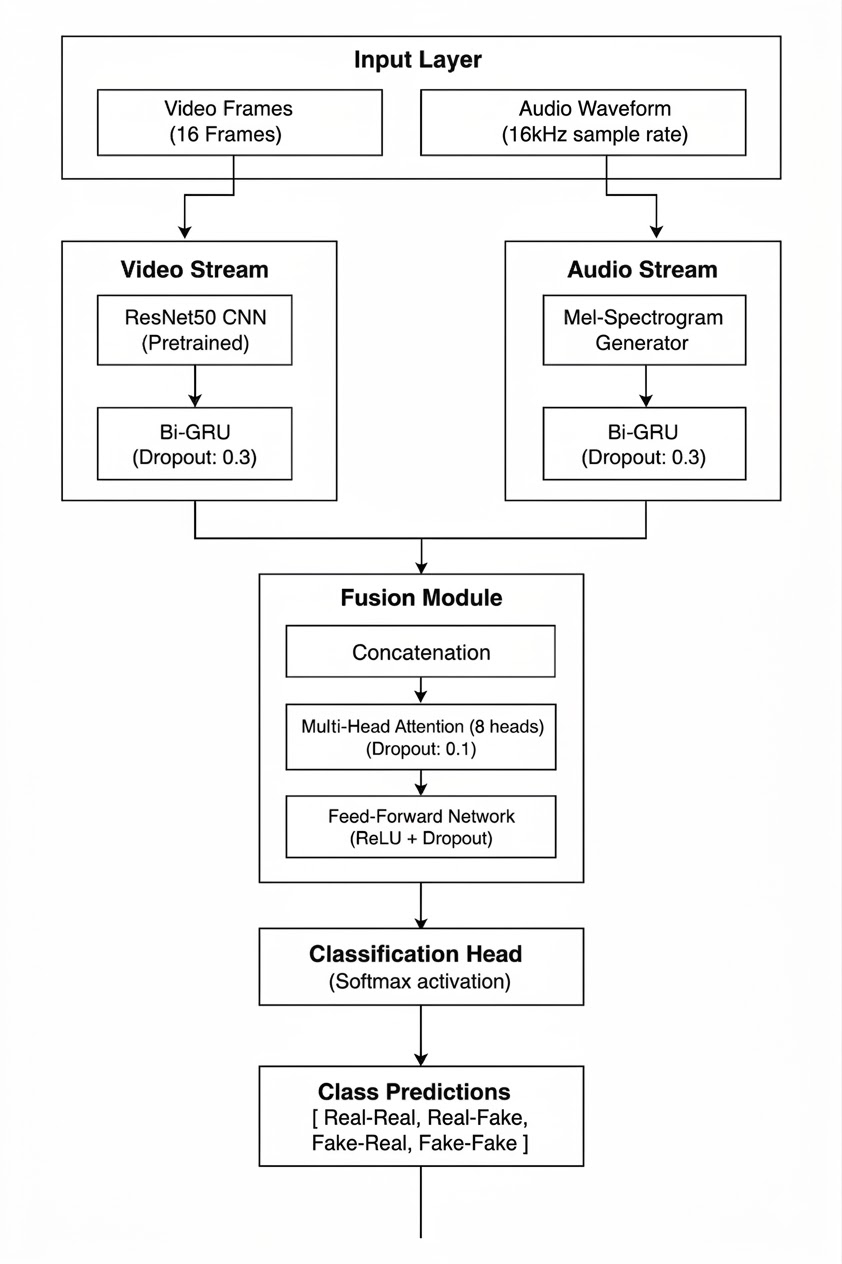
\includegraphics[width=0.95\linewidth]{diagrams/paper2_architecture.png}
\caption{Proposed dual-stream multimodal architecture with cross-modal attention fusion.}
\label{fig:phase2-arch}
\end{figure}

% Why synchrony matters: speech co-articulation imposes timing constraints that forgeries fail to replicate uniformly
\section{Biological and Forensic Motivation}
Human speech production exhibits consistent co-articulation patterns: facial articulation (visemes) typically precedes or co-occurs with corresponding phoneme acoustics within tight temporal windows. Generative pipelines trained on separate objectives for audio and video may achieve perceptual coherence but struggle to reproduce fine-grained, biologically plausible lags and coarticulation dynamics uniformly. Modeling bidirectional temporal context with explicit cross-modal attention helps detect these subtle asynchronies, which often persist even when spatial and spectral artifacts are minimized \cite{haliassos2021lips}.

% Training details: objective, optimizer, regularization, and stability techniques; keep math minimal and implementation-focused
\section{Training Protocol and Optimization}
The multimodal system is trained for the four-class task over RR, RF, FR, and FF, with binary summaries obtained by grouping RF, FR, and FF as manipulated. The accompanying paper emphasizes comparative evaluation of the full cross-modal attention model against audio-only, video-only, and simple-concatenation alternatives on the consolidated dataset.

% Evaluation design: demographic stratification and compression robustness to reflect deployment realities
\section{Fairness and Robustness Evaluation Design}
Evaluation additionally includes robustness under lossy compression and a demographic fairness analysis on FakeAVCeleb. The accompanying study reports subgroup variance below approximately 2.0\% and compares the proposed model against audio-only, video-only, and simple-concatenation baselines.

% Recap: summarizes the multimodal design and connects forward to experimental validation in Chapter~\ref{ch:experiments}
\section{Summary}
The proposed synchronicity-aware framework integrates modality-specific encoders and bidirectional temporal modeling with cross-modal attention to detect fine-grained audio–visual asynchronies characteristic of modern multimodal deepfakes. The architecture is trained with multi-class supervision to distinguish cross-modal manipulation categories and is evaluated for accuracy, robustness under compression, and fairness across demographic subgroups. Experimental results are presented in Chapter~\ref{ch:experiments} and compared against unimodal and naive fusion baselines.